\section{REQUIREMENTS}
\subsection{External Interfaces}
Here are shown some mockup that should represent an idea of the structure of the web and mobile interfaces

\subsubsection{Web User interfaces}
\begin{itemize}
\item \textbf{Visitor home page} \\ \\ This is the first page that every visitor will get. It's the homepage of myTaxiService and it allows visitors to login or register.
\begin{figure}[h]
	\centering	
	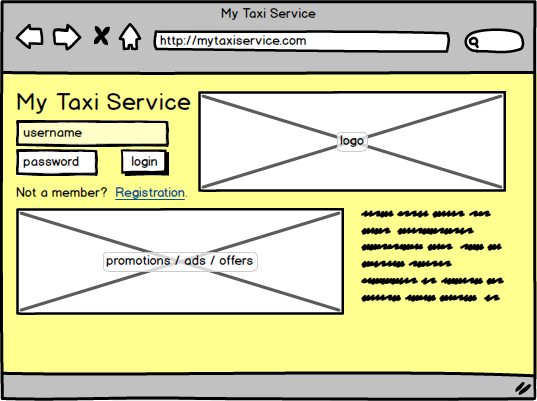
\includegraphics[width=1.05\textwidth]{web_vis}
\end{figure}

\newpage\item \textbf{Registration Form} \\  This mock shows the basic fields that the server needs to register a new user, some of them are mandatory and there could be more in future implementations. \\ \\
\begin{figure}[h]
	\centering	
	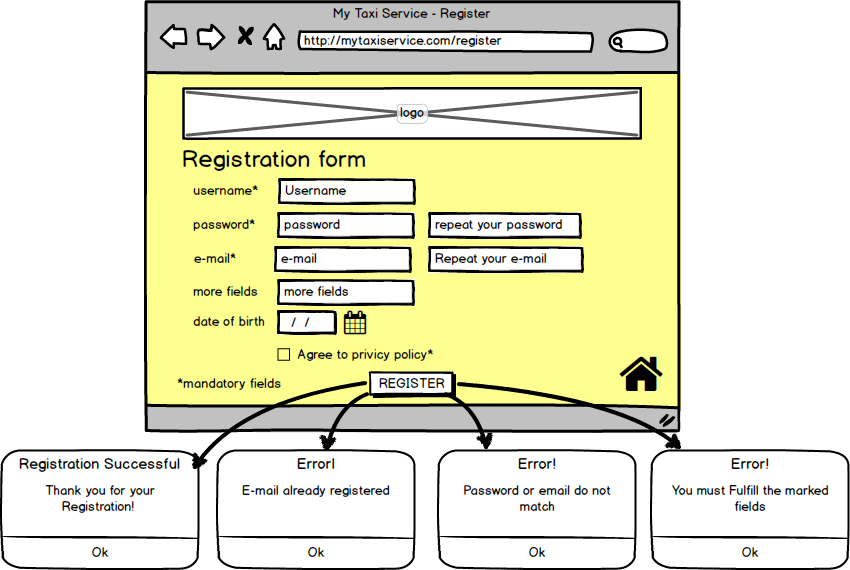
\includegraphics[width=1.2\textwidth]{web_reg}
\end{figure}

\newpage
\item \textbf{Passengers home page} \\  Registered users that have a passenger account will be lead here from the visitor home page. This mock shows the actions that they will be able to do: requesting a ride, reserving a taxi, finding a shared ride, going in the reservations page, logging out. \\ \\
\begin{figure}[h]
	\centering	
	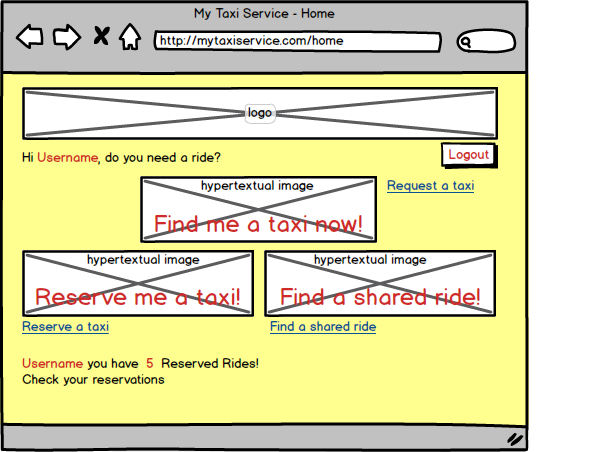
\includegraphics[width=1.2\textwidth]{web_home1}
\end{figure}
\newpage

\item \textbf{Passengers with a request home page} \\ Passengers that already have a request active and are waiting for a taxi will have a different home page, that will not allow them to do another request. \\ \\
\begin{figure}[h]
	\centering	
	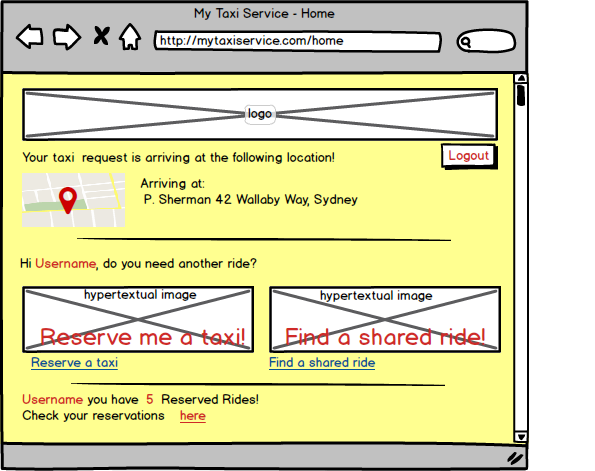
\includegraphics[width=1.2\textwidth]{web_home2}
\end{figure}
\newpage

\item \textbf{Request form} \\ This is a simply and basic mock that allows the passenger to instantly call a taxi. the system will wait for the answer of a driver \\ \\
\begin{figure}[h]
	\centering	
	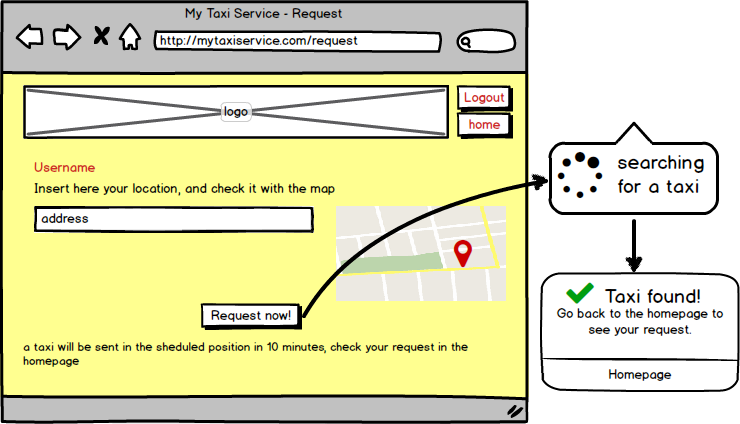
\includegraphics[width=1.2\textwidth]{web_req}
\end{figure}
\newpage

\item \textbf{Reservation Form} \\ Here is an example of how reservations should be done. They all are mandatory except for the shared ride option. \\ \\
\begin{figure}[h]
	\centering	
	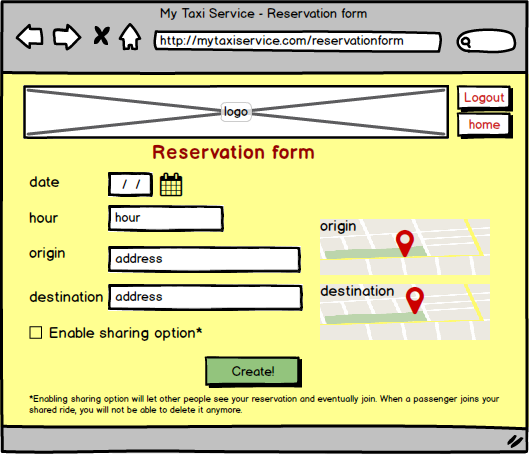
\includegraphics[width=1.2\textwidth]{web_res1}
\end{figure}
\newpage

\item \textbf{Reservations} \\ Once a reservation is done, the user is able to see it in the reservation page. they are ordered by date and hour and all the properties are listed. The example shows all the typologies of reservations, including the deletable and the not deletable ones. \\ \\
\begin{figure}[h]
	\centering	
	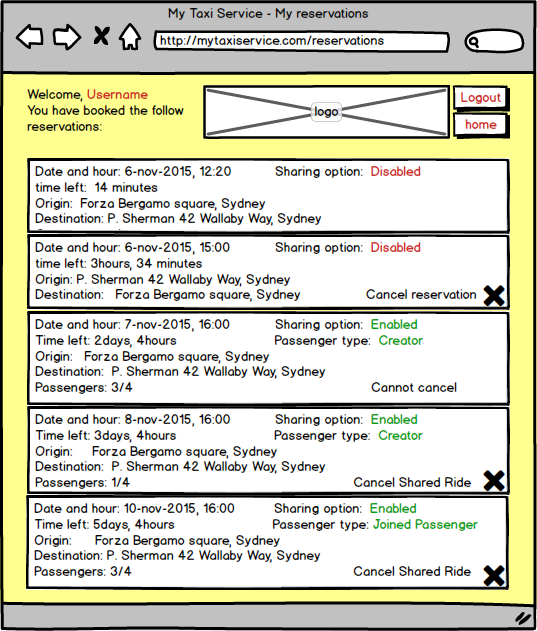
\includegraphics[width=1\textwidth]{web_res2}
\end{figure}
\newpage

\item \textbf{Shared rides} \\ This mock is the template of the shared ride page. All the fields are mandatory, after filling them, there will be shown the result of the search. The user then can join his preferred ride. \\ \\
\begin{figure}[h]
	\centering	
	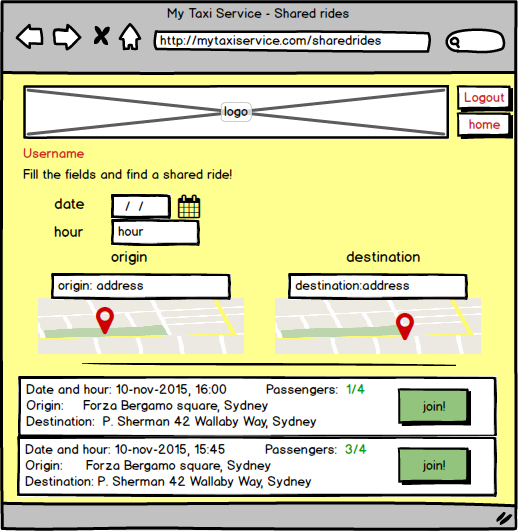
\includegraphics[width=1.1\textwidth]{web_share}
\end{figure}
\newpage
	
	
\end{itemize}












\subsection{Functional Requirements}
By analyzing the goals we came up with a list of requirements in order to achieve them:
	\begin{itemize}
		\item {[G1]} Allow a visitor to register in the system and adding/managing his information.
			\begin{itemize}
				\item {[R1]} The system will provide a registration functionality.
				\item {[R2]} System should check that user name must be unique, there cannot be two users with the same user name in the system.
				\item {[R3]} System will not allow visitors to see other pages than the login page.
				\item {[R4]} System will grant visitors access only to registration functionality.
			\end{itemize}
		\item {[G2]} Allow a user to log in to application, either he is a passenger or a taxi driver.
			\begin{itemize}
				\item {[R1]} The system will provide a log-in functionality.
				\item {[R2]} System will check that the tuple username-password inserted by the user exists in the database.
			\end{itemize}
		\item {[G3]} Allow a passenger to make a request for a taxi.
	\begin{itemize}
		\item {[R1]} The system will not grant access to this functionality if the user is not logged in.
		\item {[R2]} The system will forward a taxi request to a driver only if:
		\begin{itemize}
			\item The passenger provides a valid location for a taxi.
			\item Passenger is not waiting for another taxi called by a previous request.
			\item Passenger does not have a reserved ride occurring within thirty minutes.
		\end{itemize}
	\end{itemize}
		\item {[G4]} Allow a passenger to make a reservation for a taxi and share the ride if he wants.
			\begin{itemize}
				\item {[R1]} The system won't grant access to this functionality if the user is not logged in.
				\item {[R2]} The system will accept the reservation if the passenger: 
				\begin{itemize}
					\item Specifies starting position, destination and leaving time of the ride
					\item Completes the reservation two hours before the ride occurs.
					\item Did not make a reservation for a ride that occurs thirty minutes before or after the requested time.					
				\end{itemize}
				\item {[R3]} If a user wants to share a ride the system will permit him to enable sharing option at the moment of the reservation, then wait until the taxi is full or until 10 minutes before the scheduled time for other users to join the ride and finally compute a path for the ride.
				\item {[R4]} If the reservation is successful the system will call for a taxi via a normal request 10 minutes before the scheduled time, send a notification to the passenger, calculate the length and the cost of the ride and communicate it to all participants and to the taxi driver as well.
			\end{itemize}
		\item {[G5]} Allow a passenger to join a shared ride.
			\begin{itemize}
				\item {[R1]} The system won't grant access to this functionality if the user is not logged in.
				\item {[R2]} If a passenger wants to join a shared ride the system will ask him the starting position and destination he's headed, show all the possible non full rides heading in the same direction, wait for user decision and then add the user to the shared ride.
			\end{itemize}
		\item {[G6]} Allow a passenger to cancel a reservation/shared ride.
			\begin{itemize}
				\item {[R1]} System will not allow a passenger to cancel a ride if it will occur in less than thirty minutes.
				\item {[R2]} The system will reject a cancel request of a shared ride if someone has already joined it.
			\end{itemize}
		\item {[G7]} Allow a user to leave a shared ride.
			\begin{itemize}
				\item {[R1]} The system will allow a passenger to leave a shared ride if it won't occur within fifteen minutes.
			\end{itemize}
		\item {[G8]} Allow a taxi driver to set his availability.
			\begin{itemize}
				\item {[R1]} System will provide an interface to taxi drivers where they can notify the system that they are able to take care of a request.
			\end{itemize}
		\item {[G9]} Allow a taxi driver to accept or refuse a call for a taxi-request from the system.
			\begin{itemize}
				\item {[R1]} When a request occur the system will show a screen to the driver in which he can accept or refuse the call.
			\end{itemize}
		\item {[G10]} Provide a fair management of taxi queues.
			\begin{itemize}
				\item {[R1]} The system will divide the city in zones of two squared kilometers and will assign to each of them a certain number of taxis organized in a queue.
				\item {[R2]} The system knows at every time which taxis are assigned to a zone by using a gps system installed on the vehicles.
				\item {[R3]} When a request arrive from a zone the system will call the first taxi in the queue associated to that zone, the system will never skip to the second position in the queue.
				\item {[R4]} If a taxi refuse a request the system will place it at the and of the queue and forward the request to the second tax in the queue.S
				\item {[R3]} When a request arrive from a zone the system will call the first taxi in the queue associated to that zone.
				\item {[R4]} If a taxi refuse a request the system will place it at the end of the queue and forward the request to the second tax in the queue.

			\end{itemize}
		\end{itemize}
\newpage
\subsection{Non Functional Requirements}
	\subsubsection{Performance Requirements} Performance should be high to guarantee usability knowing that there will be a lot of real time request and computation. We assume that the response time of application is close to zero so the speed of the whole system depends only on user's internet connection.
	\subsubsection{Software System Characteristics}
		\paragraph{Availability} \hfill \\ Everyone should be able to access the application online everytime, this means that a dedicated server could be necessary.
		\paragraph {Maintainability} \hfill \\ The application will be accurately documented to help future developers in maintain and apply changes to the code.
		\paragraph{Portability} \hfill \\  The application should be compatible to all major hardware and software platform present on the market.
		\paragraph{User friendliness} \hfill \\ The application does not expect an expert user so the interface will be simple and intuitive. 
	\subsubsection{Data integrity, consistency and availability} The data should be always accessible. They should also be duplicated in case of a system fault to prevent data losses.